\documentclass[aspectratio=169]{../latex_main/tntbeamer}  % you can pass all options of the beamer class, e.g., 'handout' or 'aspectratio=43'
\usepackage{dsfont}
\usepackage{bm}
\usepackage[english]{babel}
\usepackage[T1]{fontenc}
%\usepackage[utf8]{inputenc}
\usepackage{graphicx}
\graphicspath{ {./figures/} }
\usepackage{algorithm}
\usepackage[ruled,vlined,algo2e,linesnumbered]{algorithm2e}
\usepackage{hyperref}
\usepackage{booktabs}
\usepackage{mathtools}

\usepackage{amsmath,amssymb}

\DeclareMathOperator*{\argmax}{arg\,max}
\DeclareMathOperator*{\argmin}{arg\,min}

\usepackage{amsbsy}
\newcommand{\vect}[1]{\bm{#1}}
%\newcommand{\vect}[1]{\boldsymbol{#1}}

\usepackage{pgfplots}
\pgfplotsset{compat=1.16}
\usepackage{tikz}
\usetikzlibrary{trees} 
\usetikzlibrary{shapes.geometric}
\usetikzlibrary{positioning,shapes,shadows,arrows,calc,mindmap}
\usetikzlibrary{positioning,fadings,through}
\usetikzlibrary{decorations.pathreplacing}
\usetikzlibrary{intersections}
\pgfdeclarelayer{background}
\pgfdeclarelayer{foreground}
\pgfsetlayers{background,main,foreground}
\tikzstyle{activity}=[rectangle, draw=black, rounded corners, text centered, text width=8em]
\tikzstyle{data}=[rectangle, draw=black, text centered, text width=8em]
\tikzstyle{myarrow}=[->, thick, draw=black]

% Define the layers to draw the diagram
\pgfdeclarelayer{background}
\pgfdeclarelayer{foreground}
\pgfsetlayers{background,main,foreground}

% Requires XeLaTeX or LuaLaTeX
%\usepackage{unicode-math}

\usepackage{fontspec}
%\setsansfont{Arial}
\setsansfont{RotisSansSerifStd}[ 
Path=../latex_main/fonts/,
Extension = .otf,
UprightFont = *-Regular,  % or *-Light
BoldFont = *-ExtraBold,  % or *-Bold
ItalicFont = *-Italic
]
\setmonofont{Cascadia Mono}[
Scale=0.8
]

% scale factor adapted; mathrm font added (Benjamin Spitschan @TNT, 2021-06-01)
%\setmathfont[Scale=1.05]{Libertinus Math}
%\setmathrm[Scale=1.05]{Libertinus Math}

% other available math fonts are (not exhaustive)
% Latin Modern Math
% XITS Math
% Libertinus Math
% Asana Math
% Fira Math
% TeX Gyre Pagella Math
% TeX Gyre Bonum Math
% TeX Gyre Schola Math
% TeX Gyre Termes Math

% Literature References
\newcommand{\lit}[2]{\href{#2}{\footnotesize\color{black!60}[#1]}}

%%% Beamer Customization
%----------------------------------------------------------------------
% (Don't) Show sections in frame header. Options: 'sections', 'sections light', empty
\setbeamertemplate{headline}{empty}

% Add header logo for normal frames
\setheaderimage{
	% 
\includegraphics[height=\logoheight]{figures/TNT_darkv4.pdf}
	
\includegraphics[height=\logoheight]{../latex_main/figures/luh_logo_rgb_0_80_155.pdf}
	% 
\includegraphics[height=\logoheight]{figures/logo_tntluh.pdf}
}

% Header logo for title page
\settitleheaderimage{
	% 
\includegraphics[height=\logoheight]{figures/TNT_darkv4.pdf}
	
\includegraphics[height=\logoheight]{../latex_main/figures/luh_logo_rgb_0_80_155.pdf}
	% 
\includegraphics[height=\logoheight]{figures/logo_tntluh.pdf}
}

% Title page: tntdefault 
\setbeamertemplate{title page}[tntdefault]  % or luhstyle
% Add optional title image here
%\addtitlepageimagedefault{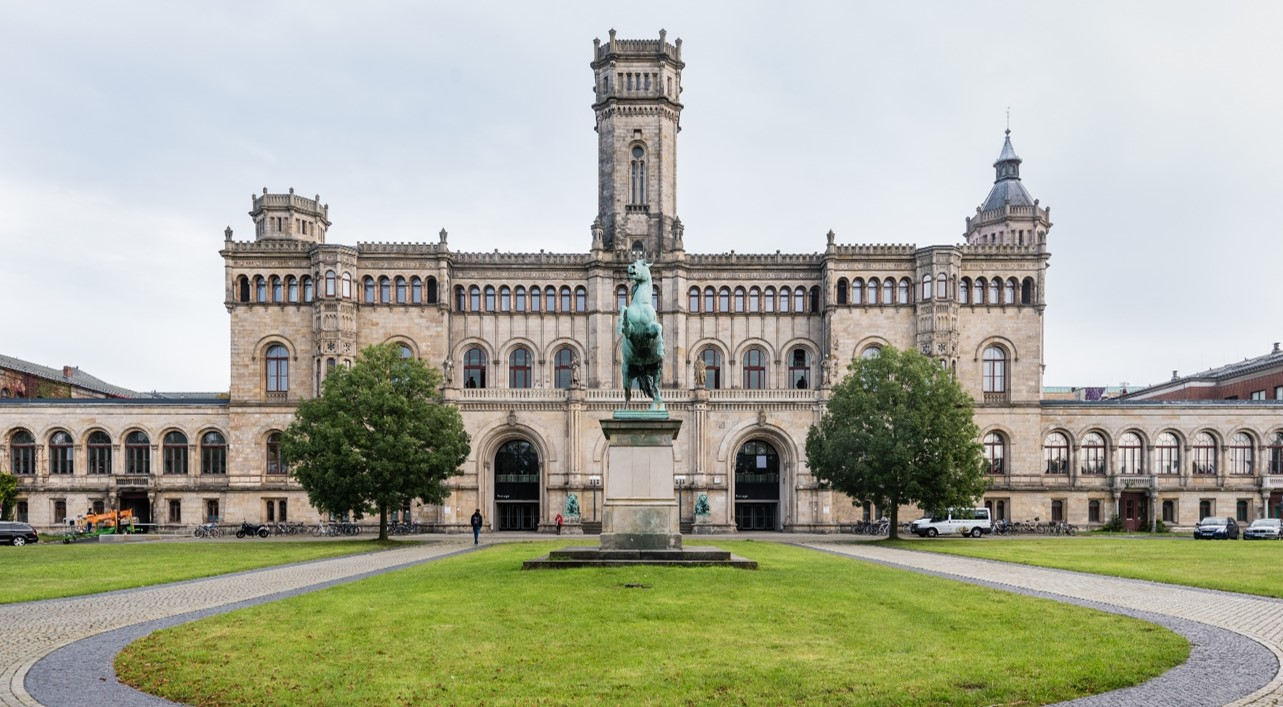
\includegraphics[width=0.65\textwidth]{figures/luh_default_presentation_title_image.jpg}}

% Title page: luhstyle
% \setbeamertemplate{title page}[luhstyle]
% % Add optional title image here
% \addtitlepageimage{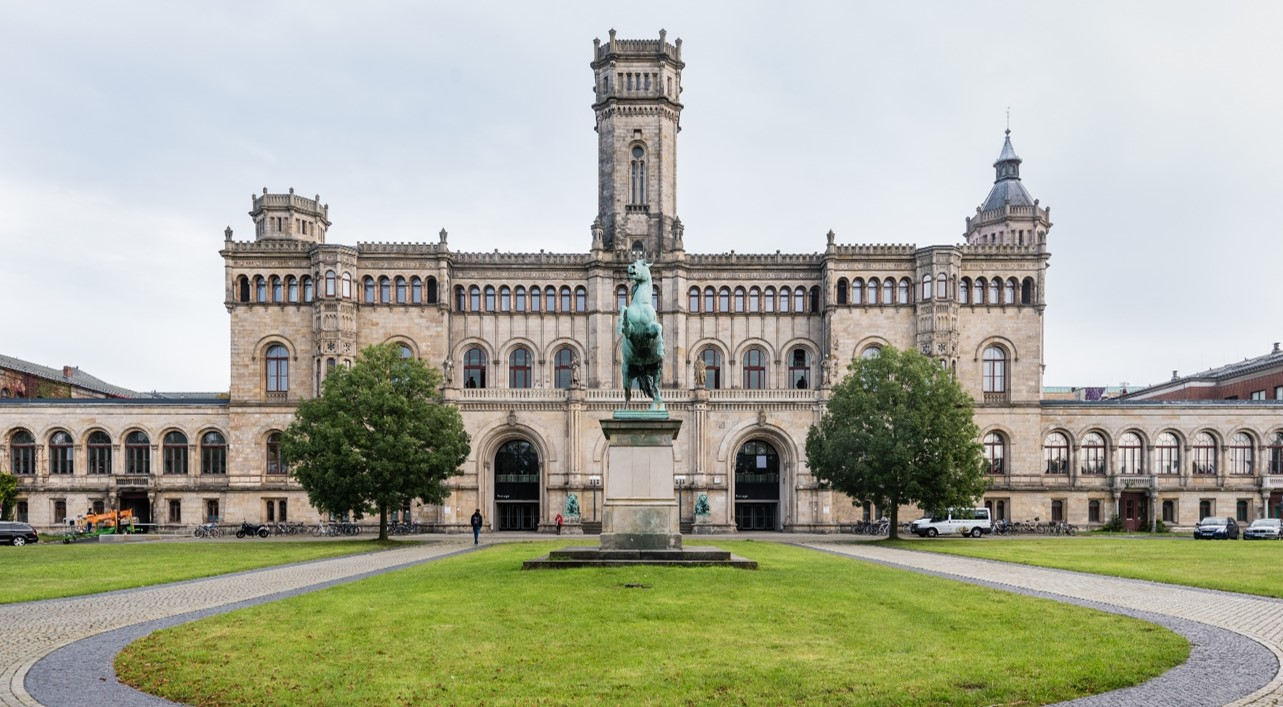
\includegraphics[width=0.75\textwidth]{figures/luh_default_presentation_title_image.jpg}}

\author[Abedjan \& Lindauer]{Ziawasch Abedjan \& Marius Lindauer\\[1em]
	
\includegraphics[height=\logoheight]{../latex_main/figures/luh_logo_rgb_0_80_155.pdf}\qquad
	
\includegraphics[height=\logoheight]{../latex_main/figures/DBIS_Kurzlogo.png}\qquad

\includegraphics[height=\logoheight]{../latex_main/figures/TNT_darkv4}\qquad

\includegraphics[height=\logoheight]{../latex_main/figures/L3S.jpg}	}
\date{Summer Term 2022; \hspace{0.5em} {
\includegraphics[height=1.5em]{../latex_main/figures/Cc-by-nc-sa_icon.svg.png}}; based on \href{https://ds100.org/fa21/}{[DS100]}
}


%%% Custom Packages
%----------------------------------------------------------------------
% Create dummy content
\usepackage{blindtext}

% Adds a frame with the current page layout. Just call \layout inside of a frame.
\usepackage{layout}


%%% Macros
%\renewcommand{\vec}[1]{\mathbf{#1}}
% \usepackage{bm}
%\let\vecb\bm

\title[Introduction]{DS: Principal Component Analysis}
\subtitle{Bonus}

\graphicspath{ {./figure/} }
%\institute{}


\begin{document}
	
	\maketitle
	\begin{frame}{As an aside...}
	    \begin{columns}
	        \begin{column}{.4\textwidth}
	                PCA has one goal stated two different ways:
	                \begin{itemize}
	                    \item Find directions that minimize projection error
	                    \item Find directions that maximize captured variance
	                \end{itemize}
	                \bigskip
	                Why are these two goals equivalent?
                    Maximizing variance = spreading out red dots
                    Minimizing error = making red lines short
	        \end{column}
	        
	        
	        \begin{column}{.6\textwidth}
	                \begin{figure}
	                    %\centering
	                    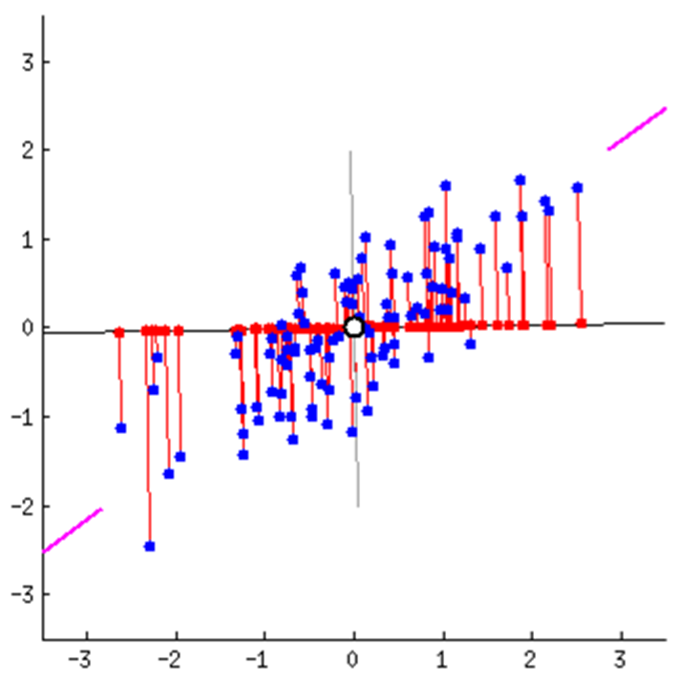
\includegraphics[scale=.25]{Bild18}
	                \end{figure}
	        \end{column}
	    \end{columns}
	    \url{https://stats.stackexchange.com/questions/2691/making-sense-of-principal-component-analysis-eigenvectors-eigenvalues/140579\#140579}

	\end{frame}
	
	\begin{frame}{As an aside...}
	    \begin{columns}
	        \begin{column}{.4\textwidth}
	                Imagine that the black line is a stick, and the red lines are springs attached to the stick from the points.\\
	                \bigskip
	                The first PC is where the stick comes to rest.\\
	                \bigskip
                    SVD finds this for us.\\
                    
	        \end{column}
	        
	        
	        \begin{column}{.6\textwidth}
	                \begin{figure}
	                    \centering
	                    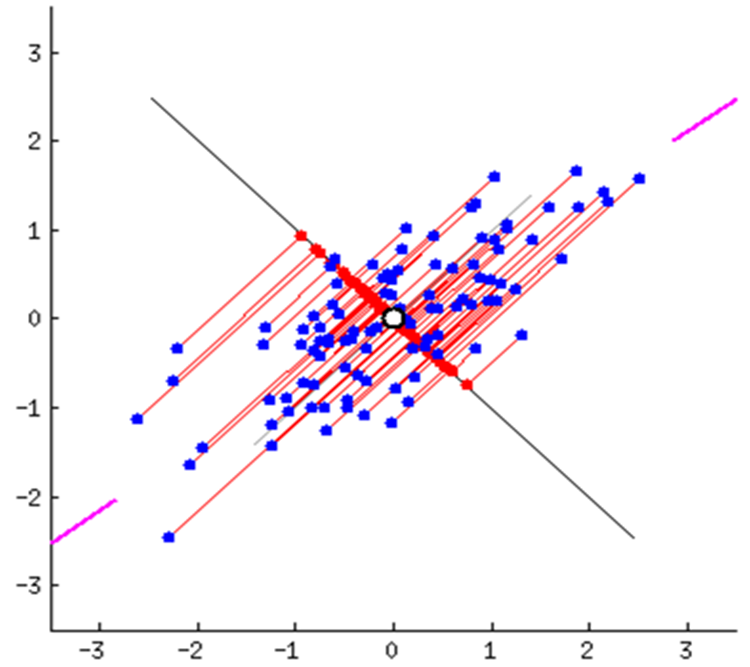
\includegraphics[scale=.25]{Bild19}
	                \end{figure}
	        \end{column}
	        
	        
	    \end{columns}
	    \url{https://stats.stackexchange.com/questions/2691/making-sense-of-principal-component-analysis-eigenvectors-eigenvalues/140579\#140579}

	\end{frame}
	
	
	\begin{frame}{Regression: The Big Idea}
	    \begin{columns}
	        \begin{column}{.5\textwidth}
	                Suppose we know the child mortality rate of a given country
	                \begin{itemize}
	                    \item Linear regression tries to predict the fertility rate from the mortality rate
	                    \item For example, if the mortality is 6, we might guess the fertility is near 4
	                \end{itemize}
	                \bigskip
	                The regression line tells us the “best” prediction of fertility given all possible mortality values\\
	                \begin{itemize}
	                    \item Minimizes the root mean squared error [see vertical red lines, only some shown]
	                \end{itemize}
	        \end{column}
	        
	        
	        \begin{column}{.5\textwidth}
	                \begin{figure}
	                    \centering
	                    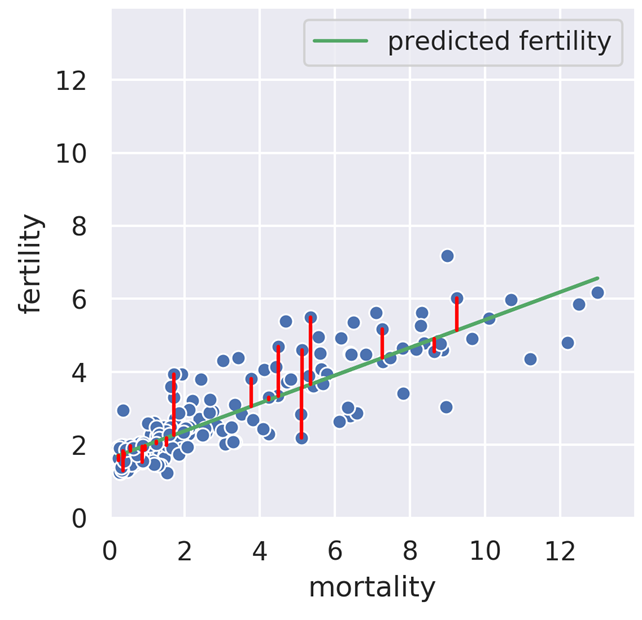
\includegraphics[scale=.5]{Bild20}
	                \end{figure}
	        \end{column}
	        
	        
	    \end{columns}

	\end{frame}
	
	
	
	\begin{frame}{Regression: The Big Idea}
	    \begin{columns}
	        \begin{column}{.5\textwidth}
	                We can also perform a regression in the reverse direction.\\
	                \bigskip
	                That is, given the fertility, we try to predict the mortality.\\
	                \bigskip
	                In this case, we get a different regression line which minimizes the root mean squared length of the horizontal lines.
	        \end{column}
	        
	        
	        \begin{column}{.5\textwidth}
	                \begin{figure}
	                    \centering
	                    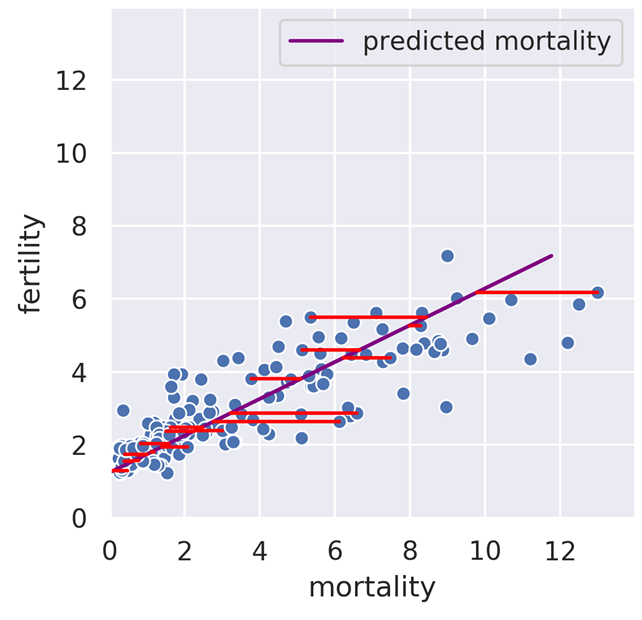
\includegraphics[scale=.5]{Bild21}
	                \end{figure}
	        \end{column}
	        
	        
	    \end{columns}

	\end{frame}
	
	
	\begin{frame}{SVD: Minimizing the Perpendicular Error}
	    \begin{columns}
	        \begin{column}{.5\textwidth}
	                Instead of minimizing horizontal or vertical error, the first principal component minimizes the error \underline{perpendicular} to the subspace onto which we’re projecting\\
	                \bigskip
	                That is, SVD finds the line such that if we project our data onto that line, the error between the projection and our original data is minimized
	        \end{column}
	        
	        
	        \begin{column}{.5\textwidth}
	                \begin{figure}
	                    \centering
	                    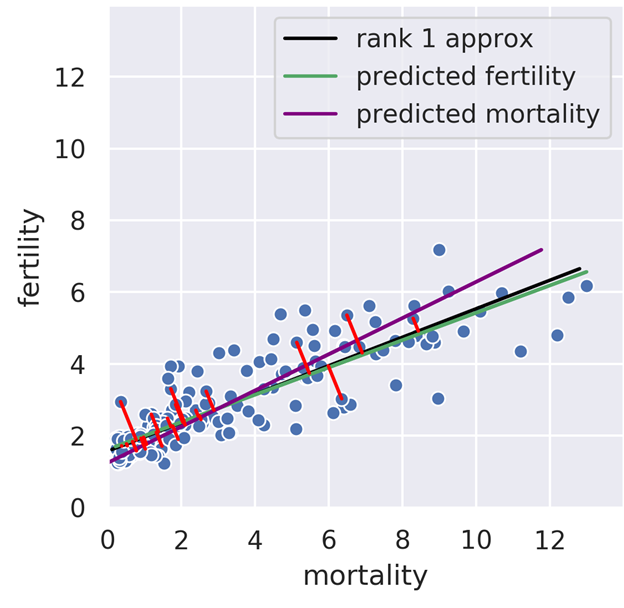
\includegraphics[scale=.5]{Bild22}
	                \end{figure}
	        \end{column}
	        
	        
	    \end{columns}

	\end{frame}
\end{document}